\documentclass[aspectratio=169]{beamer}
\usepackage[framemethod=tikz]{mdframed}
\usepackage{pgfplots}
\usepackage{tikz}
\usepackage{url}
\usepackage{xcolor}
\usepackage{xmpmulti}
\usetikzlibrary{shapes,arrows}
\hypersetup{pdfstartview={Fit}} % Fit the presentation to the window when first displayed
\usetheme{Frankfurt}
\pgfplotsset{compat=1.14}
\beamertemplatenavigationsymbolsempty{} % Remove Beamer navigation symbols
\nonstopmode{} % Keep making the file through errors
\usepackage[sfdefault]{sourcesanspro}
\usepackage[T1]{fontenc}

% http://danielfalster.com/blog/2013/06/18/a-nice-title-page-for-beamer-presentations/
\newmdenv[tikzsetting={draw=black,fill=white,fill opacity=0.7, line width=1pt},backgroundcolor=none,leftmargin=0,rightmargin=0,innertopmargin=5pt,skipbelow=\baselineskip,skipabove=\baselineskip]{TitleBox}

\title{Surfing the Radio Waves with PostgreSQL: \\ Creating Sample Datasets for Fun and Profit}
\author[Swartz]{Tom~Swartz}
\institute{Central PA Open Source Conference 2020}
\date{December 5 2020}
\subject{Computer Science}
\begin{document}

% Title Page
{\usebackgroundtemplate{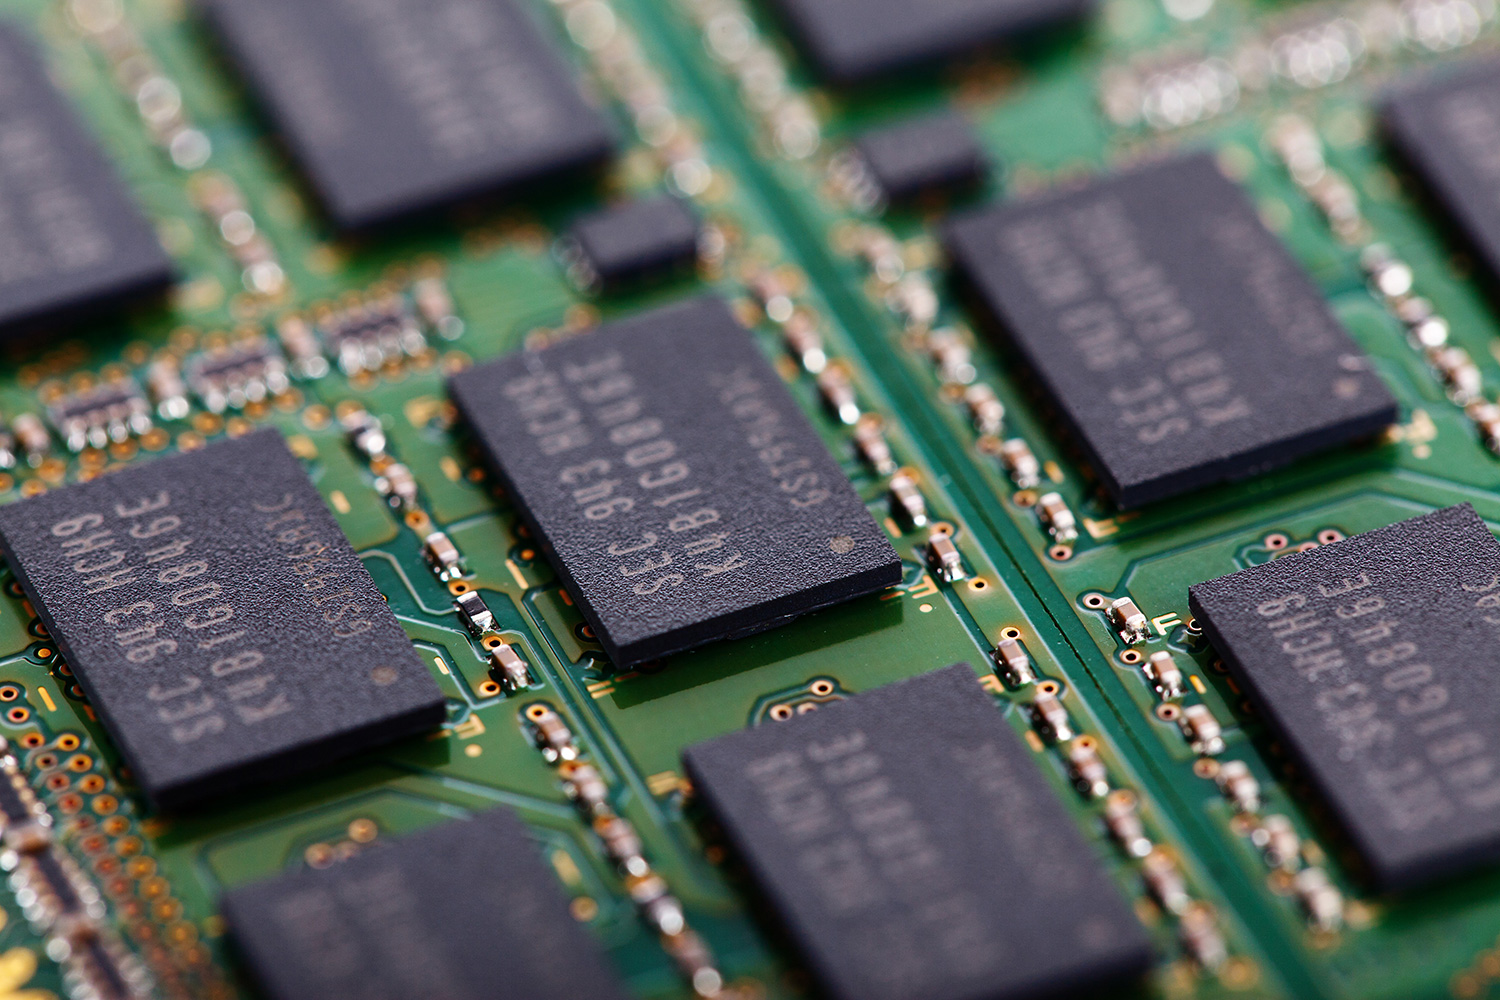
\includegraphics[width=1.00\paperwidth,keepaspectratio]{images/close-up-computer-ram.jpg}}
\begin{frame}[plain]
    \begin{TitleBox}
        \begin{center}
            {\color{red}\Large\inserttitle\color{black}}\\
        \end{center}
        \insertauthor{}\hfill\insertinstitute{}\\
        {\footnotesize
        \href{http://twitter.com/tswartz07}{@tswartz07}
        \hfill
        \href{mailto: tom@tswartz.net}{tom@tswartz.net}
        }
    \end{TitleBox}
    \vspace{15em}
\end{frame}}

\begin{frame}
  \frametitle{Who is this guy?}
  \framesubtitle{And what is he doing here?}
  \begin{columns}[T]
    \begin{column}[T]{0.45\paperwidth}
      {\huge Tom Swartz}
      \vfill
      \begin{itemize}%[<+->]
        \item{Crunchy Data Support and Development Engineering}
        \item{5 years DBA Support experience}
        \item{This topic is orthogonal to my day job and hobby projects}
        \item{Hobbyist interests in `Big Data', IoT, RF Communications}
      \end{itemize}
    \end{column}
    \begin{column}[T]{0.45\paperwidth}
      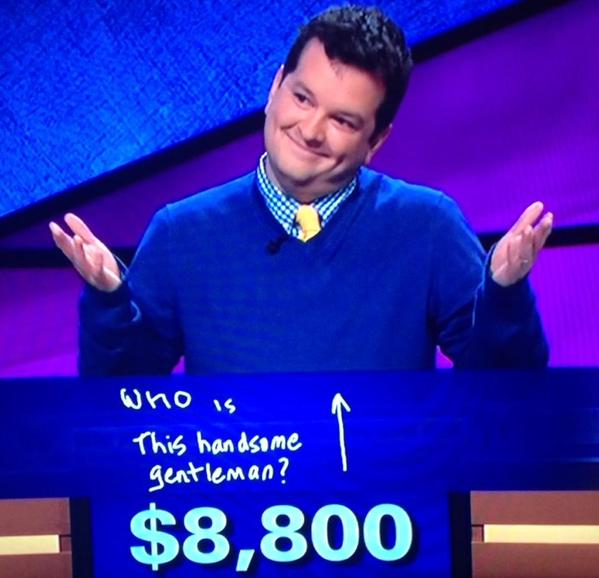
\includegraphics[height=6cm]{images/who-dat.jpg}
    \end{column}
  \end{columns}
\end{frame}

\begin{frame}[fragile]
  \frametitle{Why?}
  \begin{itemize}[<+->]
    \item{A practical application for using software and tool-sets that customers already use}
    \item{A continuous source of `free' data to be used for testing purposes}
    \item{A regular dataset that can provide value to you}
    \item{A solid use case for HomeLab equipment, for nerd cred}
 \end{itemize}
\end{frame}

\begin{frame}
  \frametitle{Summary of Applications}
  We'll be reviewing the following applications, and lessons learned from each:
  \begin{enumerate}
    \item{Weather Sensors}
    \item{Airplane Tracking}
    \item{PiHole Stats}
    \item{PA COVID-19 Data}
  \end{enumerate}
\end{frame}

\section{Introduction to SDR}
\subsection{Crash Course in SDR}
\begin{frame}
  \subsectionpage{}
\end{frame}

\begin{frame}[fragile]
    \frametitle{Software Defined Radio}
    \framesubtitle{Crash Course in SDR}
    \begin{center}
        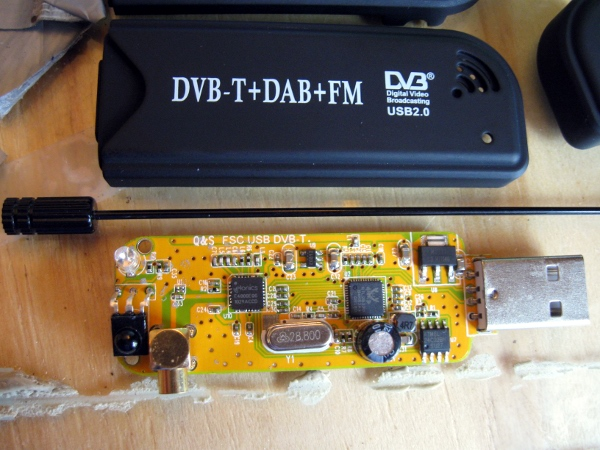
\includegraphics[width=0.75\paperwidth,height=0.75\paperheight,keepaspectratio]{images/rtlsdr.jpg}
    \end{center}
\end{frame}
\begin{frame}
    \frametitle{Software Defined Radio}
    \framesubtitle{SDR Hardware}
    \begin{columns}[T]
        \begin{column}[T]{6cm}
            \begin{itemize}
                \item{Very inexpensive device}
                \item{Uses computer software to interpret signals, rather than discrete transistors and expensive radio hardware}
                \item{Can receive 24~MHz to 2~GHz}
            \end{itemize}
        \end{column}
        \begin{column}[T]{5cm}
            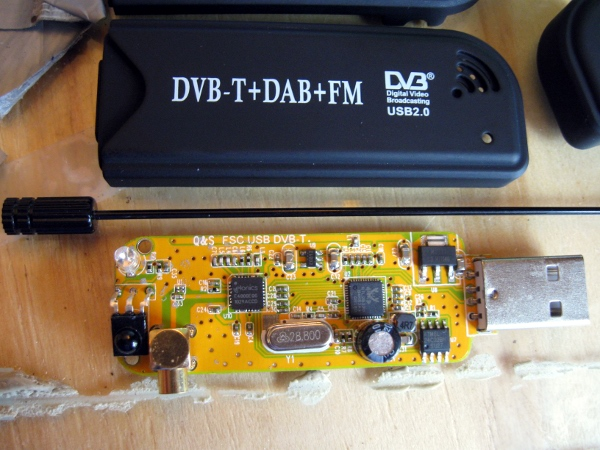
\includegraphics[height=4cm]{images/rtlsdr.jpg}
        \end{column}
    \end{columns}
\end{frame}
\begin{frame}[fragile]
    \frametitle{Frequencies}
    % https://tex.stackexchange.com/questions/98695/how-do-i-generate-a-logarithmic-x-axis-without-a-y-axis
    \begin{center}
        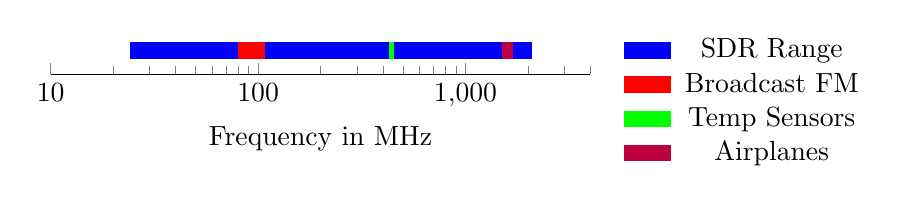
\begin{tikzpicture}
            \begin{axis}[
                    y=1.5cm,            % y unit vector
                    hide y axis,        % hide the y axis
                    legend style={draw=none},
                    legend pos=outer north east,
                    xmode = log,        % logarithmic x axis
                    axis x line*=bottom,% only show the bottom x axis line, without an arrow tip
                    log ticks with fixed point, % show layman numbers, not exponential format
                    xmin=10, xmax=4000,% range for the x axis
                    xlabel = Frequency in MHz
                ]
                \addplot [blue, no markers, line width=6pt] table {
                    24   1
                    2100 1

                };
                \addplot [red, line width=6pt] table {
                    80 1
                    108 1
                };
                \addplot [green, line width=6pt] table {
                    430 1
                    450 1
                };
                \addplot [purple, line width=6pt] table {
                    1500 1
                    1700 1
                };
                \legend{SDR Range, Broadcast FM, Temp Sensors, Airplanes}
            \end{axis}
        \end{tikzpicture}
        \begin{description}
          \item[RTL-SDR Range]\dotfill 24~MHz $\to$ 2100~MHz
            \item[Broadcast FM]\dotfill 88~MHz $\to$ 108~MHz
            \item[Remote Temperature Sensors]\dotfill 433~MHz
            \item[Airplane Tracking]\dotfill 1090~MHz
        \end{description}
    \end{center}
\end{frame}
\begin{frame}[plain]
    \frametitle{Software Defined Radio}
    \framesubtitle{What types of things can SDR's receive?}
    \begin{itemize}
        \item Morse Code
        \item Broadcast FM Radio
        \item IoT Devices
        \item Tire Pressure Monitoring Sensors
        \item Amateur Radio
        \item Ship Tracking
        \item Baby Monitors
        \item Weather Balloons
        \item GPS Signals
        \item GSM Cell Phone Signals
        \item Aircraft Tracking
        \item Locomotive Tracking
        \item Taxi Dispatch
        \item \dots lots more
    \end{itemize}
\end{frame}
\begin{frame}[fragile]
  \begin{center}
  
\includegraphics[width=0.75\paperwidth]{images/planes-trains.jpeg}
  \end{center}
\end{frame}

\subsection{Computing Hardware}
\begin{frame}[fragile]
    \frametitle{Software Defined Radio}
    \framesubtitle{Open Source Software for Satellites}
    \begin{enumerate}
        \item A program to receive/record the signal
            \begin{itemize}
                \item GQRX
                \item \verb|rtl_fm|
                \item \verb|rtl_tcp|
            \end{itemize}
        \item A program to post-process and decode the signal
            \begin{itemize}
                \item \verb|dump1090|
                \item \verb|rtl_433|
                \item ADS/B Exchange
            \end{itemize}
        \item A program to aggregate and graph the data
            \begin{itemize}
                \item PostGIS
                \item Grafana
            \end{itemize}
    \end{enumerate}
\end{frame}
\begin{frame}[fragile]
  \frametitle{The Hardware:}
  \begin{columns}[T]
    \begin{column}[T]{0.5\paperwidth}
      PostgreSQL on 2 Raspberry Pi 3B+
      \begin{itemize}
        \item{1GB RAM}
        \item{1.4 GHz ARM Processor}
        \item{Only \$35!}
        \item{28 GB Database? No sweat}
      \end{itemize}
      \vfill
      Provides endless `fun' in building software for ARM32, limited hardware, and
      providing a platform to test software used by my company and customers.
    \end{column}
    \begin{column}[T]{0.45\paperwidth}
      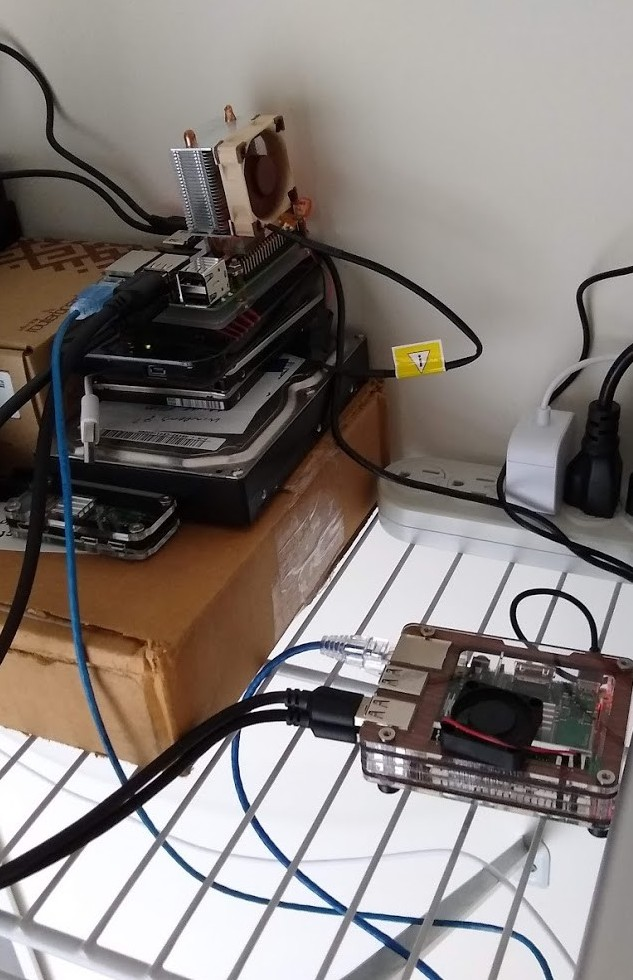
\includegraphics[height=6cm]{images/datacloset.jpg}
    \end{column}
  \end{columns}
\end{frame}

\section{Weather Sensors}
\frame{\sectionpage}
\subsection{Introduction}

\begin{frame}[fragile]
  \frametitle{Weather Sensors}
  \framesubtitle{Problem-Driven Solution}
  \begin{columns}[T]
    \begin{column}[T]{0.5\paperwidth}
      \begin{enumerate}
        \item{Base stations were limited}
        \item{Only display 24h results}
        \item{No long term historical data}
        \item{No reporting}
        \item{Base-station models which offer reporting are \$\$\$}
      \end{enumerate}
    \end{column}
    \begin{column}[T]{0.45\paperwidth}
      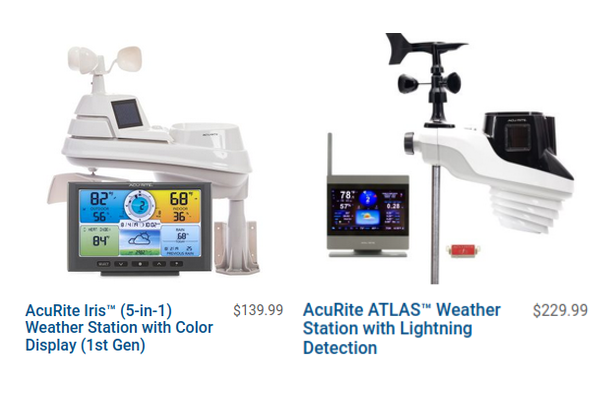
\includegraphics[width=0.45\paperwidth]{images/cost.png}
    \end{column}
  \end{columns}
\end{frame}

\begin{frame}[fragile]
  \begin{center}
  
\includegraphics[height=0.75\paperheight]{images/bender.jpg}
  \end{center}
\end{frame}

\begin{frame}[plain,fragile]
  \frametitle{Data Flow}
  % Flowchart styles
  \tikzstyle{decision} = [diamond, draw, fill=green!20, text width=4.5em, text badly centered, node distance=3cm, inner sep=0pt]
  \tikzstyle{block} = [rectangle, draw, fill=blue!20, text width=5em, text centered, rounded corners, minimum height=4em]
  \tikzstyle{line} = [draw, -latex']
  \tikzstyle{cloud} = [draw, ellipse,fill=red!20, node distance=3cm, minimum height=2em]

  \begin{tikzpicture}[node distance = 2cm, auto]
    % Draw blocks
    \node [cloud] (init) {Remote sensor};
    \node [block, below of=init] (identify) {RTL-SDR Receives data};
    \node [block, below of=identify] (evaluate) {\verb|rtl_433| decode};
    \node [block, right of=identify, node distance=3cm] (etl) {PostgreSQL Python Adapter};
    \node [decision, right of=etl] (db) {Weather Database};
    \node [block, right of=db, node distance=3cm] (grafana) {Grafana};
    \node [cloud, above of=grafana] (browser) {Remote Browser};
    % Draw connections
    \path [line,dashed] (init) -- (identify);
    \path [line] (identify) -- (evaluate);
    \path [line] (evaluate) -| (etl);
    \path [line] (etl) -- (db);
    \path [line] (grafana) -- (db);
    \path [line,dashed] (browser) -- (grafana);
  \end{tikzpicture}
\end{frame}

\begin{frame}[fragile]
  \frametitle{Issues and Lessons Learned}
  \begin{enumerate}
    \item{Good DB design should not be an afterthought}
    \item{JSONB is good, but not as good as native tables}
    \item{Indexes are really necessary}
    \item{\verb|work_mem| tweaks really pay off}
    \item{Good lessons about data de-duplication}
  \end{enumerate}
\end{frame}

\section{Airplane Tracking}
\frame{\sectionpage}
\subsection{Introduction}

\begin{frame}[fragile]
  \begin{center}
  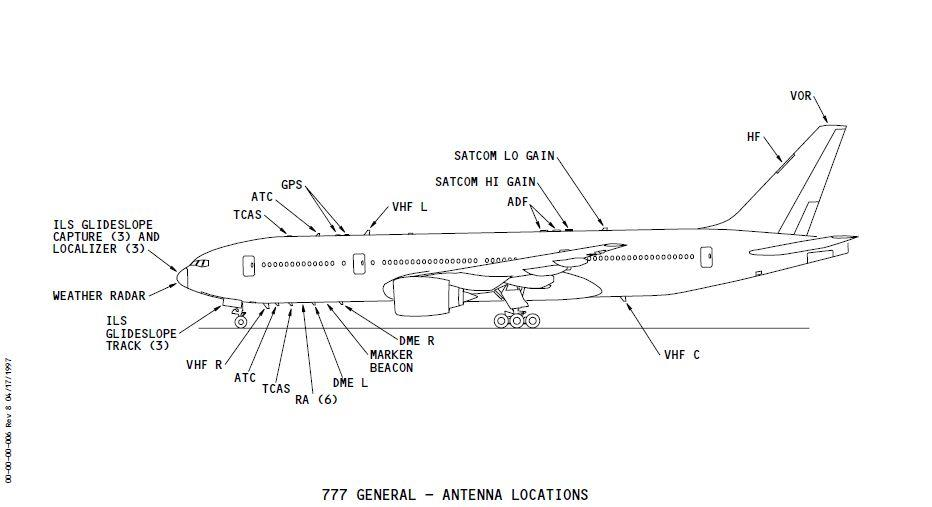
\includegraphics[height=0.70\paperheight]{images/adsb-plane.jpg}
  \end{center}
\end{frame}

\begin{frame}[plain,fragile]
  \frametitle{Data Flow}
  % Flowchart styles
  \tikzstyle{decision} = [diamond, draw, fill=green!20, text width=4.5em, text badly centered, node distance=3cm, inner sep=0pt]
  \tikzstyle{block} = [rectangle, draw, fill=blue!20, text width=5em, text centered, rounded corners, minimum height=4em]
  \tikzstyle{line} = [draw, -latex']
  \tikzstyle{cloud} = [draw, ellipse,fill=red!20, node distance=3cm, minimum height=2em]

  \begin{tikzpicture}[node distance = 2cm, auto]
    % Draw blocks
    \node [cloud] (init) {Airplane broadcast};
    \node [block, below of=init] (identify) {RTL-SDR Receives data};
    \node [block, below of=identify] (evaluate) {\verb|dump1090| decode};
    \node [block, right of=identify, node distance=3cm] (etl) {PostgreSQL Python Adapter};
    \node [decision, right of=etl] (db) {ADSB Database};
    \node [block, right of=db, node distance=3cm] (grafana) {Grafana};
    \node [cloud, above of=grafana] (browser) {Remote Browser};
    \node [cloud, below of=grafana] (gis) {PostGIS Viewer};
    % Draw connections
    \path [line,dashed] (init) -- (identify);
    \path [line] (identify) -- (evaluate);
    \path [line] (evaluate) -| node [anchor=north] {UDP Socket} (etl);
    \path [line] (etl) -- (db);
    \path [line] (grafana) -- (db);
    \path [line,dashed] (browser) -- (grafana);
    \path [line,dashed] (gis) -| (db);
  \end{tikzpicture}
\end{frame}

\begin{frame}
  \frametitle{Let's talk about Views}
  \framesubtitle{A brief aside\dots}
  \begin{columns}[T]
    \begin{column}[T]{0.5\paperwidth}
      A `view' in PostgreSQL is a pseudo-table which reconfigures the way data
      is presented.
      \begin{enumerate}
        \item{Can be used to simplify a complicated query}
        \item{Can be used to restructure data}
        \item{Can be used to easily restrict certain data types}
      \end{enumerate}
    \end{column}
    \begin{column}[T]{0.45\paperwidth}
      \textbf{Because much of the ADS/B data is spread across many messages, we can use
      different PostgreSQL Views to simplify inspecting the data.}
    \end{column}
  \end{columns}
\end{frame}

\begin{frame}[fragile]
  \frametitle{Issues and Lessons Learned}
  \begin{enumerate}
    \item{`Baby's First Big Data'}
    \item{Practice in rapid data processing}
    \item{Excellent use case for views}
    \item{Good lessons about data analysis}
  \end{enumerate}
\end{frame}

\section{PiHole Stats}
\begin{frame}[plain]
  \begin{center}
  \LARGE{Enough radio stuff!

  Lets talk more tangible data sources!}
  \end{center}
\end{frame}

\frame{\sectionpage}
\subsection{Introduction}
\begin{frame}[plain,fragile]
  \frametitle{Data Flow}
  % Flowchart styles
  \tikzstyle{decision} = [diamond, draw, fill=green!20, text width=4.5em, text badly centered, node distance=3cm, inner sep=0pt]
  \tikzstyle{block} = [rectangle, draw, fill=blue!20, text width=5em, text centered, rounded corners, minimum height=4em]
  \tikzstyle{line} = [draw, -latex']
  \tikzstyle{cloud} = [draw, ellipse,fill=red!20, node distance=3cm, minimum height=2em]

  \begin{tikzpicture}[node distance = 2cm, auto]
    % Draw blocks
    \node [cloud] (init) {PiHole};
    \node [block, below of=init] (identify) {PiHole API};
    \node [block, right of=identify, node distance=3cm] (etl) {PostgreSQL Python Adapter};
    \node [decision, right of=etl] (db) {PiHole Database};
    \node [block, right of=db, node distance=3cm] (grafana) {Grafana};
    \node [cloud, above of=grafana] (browser) {Remote Browser};
    % Draw connections
    \path [line,dashed] (init) -- (identify);
    \path [line] (identify) -- (etl);
    \path [line] (etl) -- (db);
    \path [line] (grafana) -- (db);
    \path [line,dashed] (browser) -- (grafana);
  \end{tikzpicture}
\end{frame}

\begin{frame}[fragile]
  \frametitle{Issues and Lessons Learned}
  \begin{enumerate}
    \item{Lessons in cross-table/cross-schema data handling}
    \item{Practice in bulk upserts}
    \item{Great dataset for practicing data retention policies}
    \item{Excellent lessons about autovacuum/statistics tuning}
  \end{enumerate}
\end{frame}

\section{PA COVID-19 Stats}
\frame{\sectionpage}
\subsection{Introduction}

\begin{frame}[plain,fragile]
  \frametitle{Data Flow}
  % Flowchart styles
  \tikzstyle{decision} = [diamond, draw, fill=green!20, text width=4.5em, text badly centered, node distance=3cm, inner sep=0pt]
  \tikzstyle{block} = [rectangle, draw, fill=blue!20, text width=5em, text centered, rounded corners, minimum height=4em]
  \tikzstyle{line} = [draw, -latex']
  \tikzstyle{cloud} = [draw, ellipse,fill=red!20, node distance=3cm, minimum height=2em]

  \begin{tikzpicture}[node distance = 2cm, auto]
    % Draw blocks
    \node [cloud] (init) {PA Dept of Health};
    \node [cloud, below of=init] (scrape) {Web page scrape};
    \node [cloud, right of=init, node distance=4cm] (nyt) {NYT Dataset};
    \node [block, right of=scrape, node distance=4cm] (etl) {PostgreSQL `load' scripts};
    \node [decision, right of=etl] (db) {COVID19 Database};
    \node [block, right of=db, node distance=3cm] (grafana) {Grafana};
    \node [cloud, above of=grafana] (browser) {Remote Browser};
    \node [cloud, below of=db] (gnuplot) {GnuPlot/GitHub Plots};
    % Draw connections
    \path [line,dashed] (init) -- (scrape);
    \path [line] (etl) -- (db);
    \path [line] (grafana) -- (db);
    \path [line,dashed] (browser) -- (grafana);
    \path [line,dashed] (nyt) -- (etl);
    \path [line, dashed] (scrape) -- (etl);
    \path [line, dashed] (db) -- (gnuplot);
  \end{tikzpicture}
\end{frame}

\begin{frame}[fragile]
  \frametitle{Issues and Lessons Learned}
  \begin{enumerate}
    \item{Great lessons in scripted updates}
    \item{Great use case for data analysis in Postgres}
    \item{Excellent lessons about bulk loading processes}
    \item{Even better lessons in tuning settings for regular large imports}
  \end{enumerate}
\end{frame}

\section{Wrapping Up}
\frame{\sectionpage}

\begin{frame}
  \frametitle{Key Takeaways}
  \begin{itemize}
    \item Creating your own source of constantly refreshing data for testing purposes is easy, inexpensive, and a great learning experience.
  \end{itemize}
\end{frame}
\begin{frame}
  \frametitle{Key Takeaways}
  \begin{itemize}
    \item Creating your own source of constantly refreshing data for testing purposes is easy, inexpensive, and a great learning experience.
    \item If nothing else, you can experiment with a variety of different data sources for PostgreSQL.
  \end{itemize}
\end{frame}

\begin{frame}
  \frametitle{Thank You}
  \begin{center}
    \LARGE{Questions?}
    \vfill
    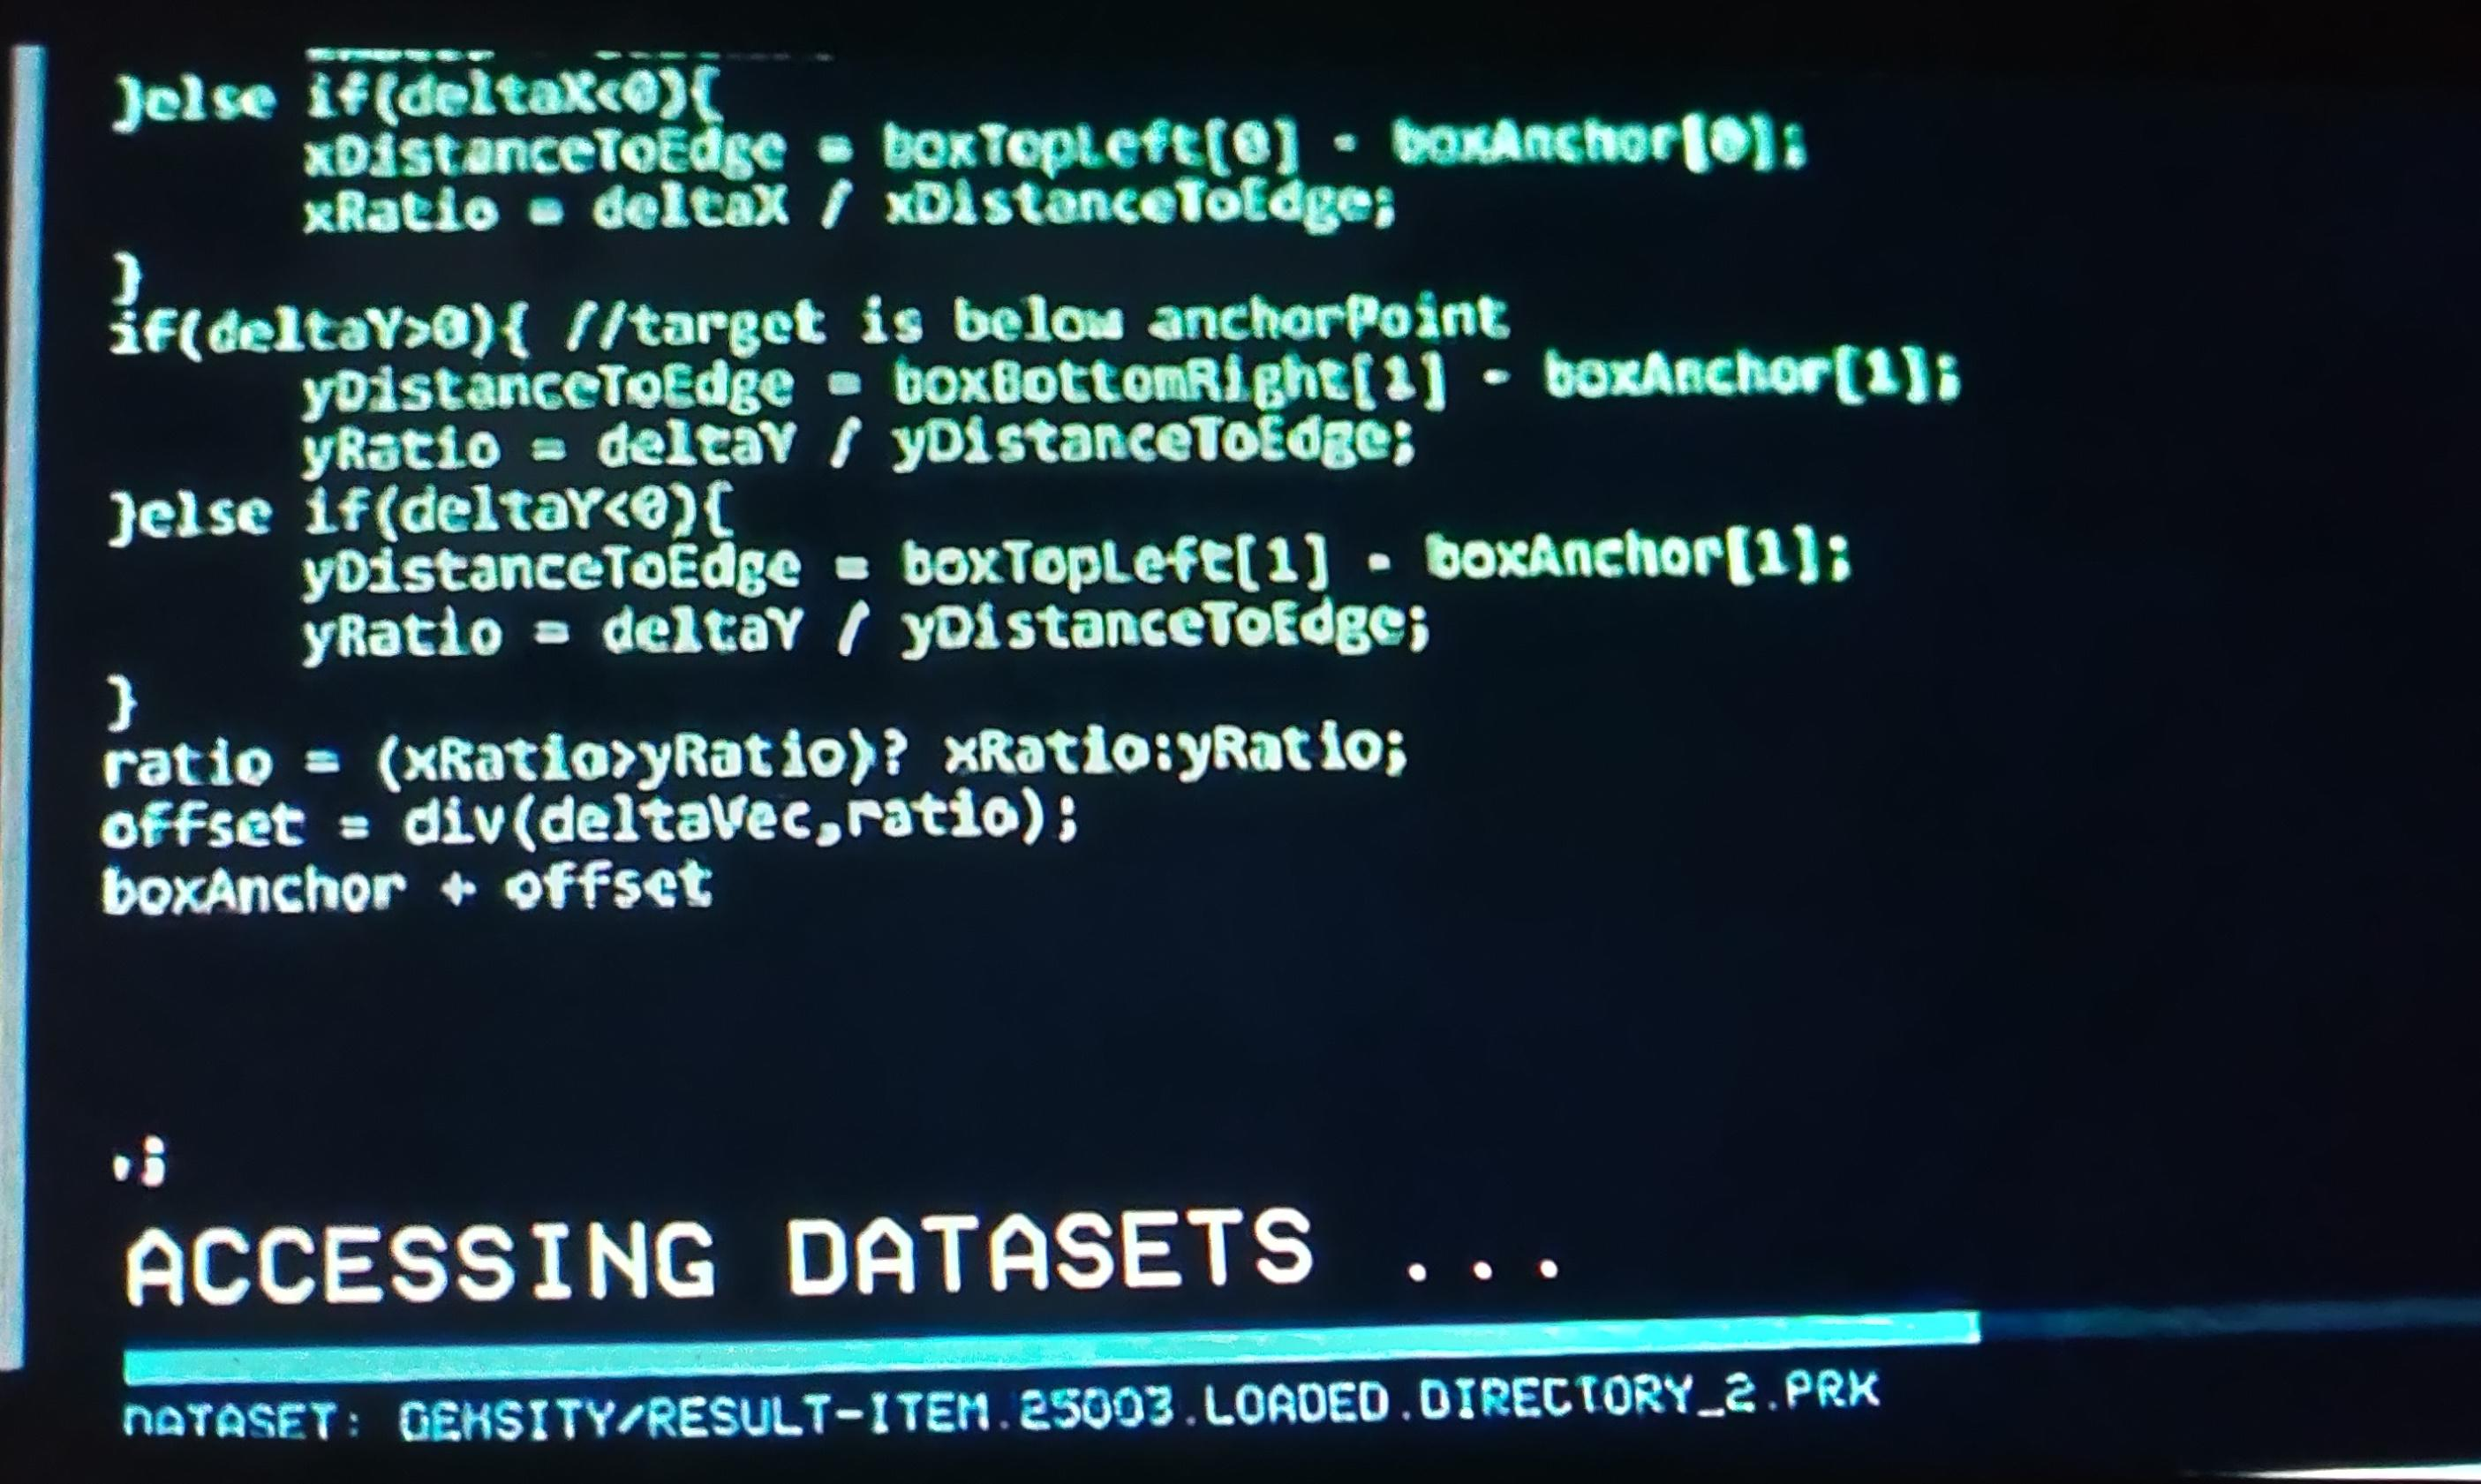
\includegraphics[height=5cm]{images/lol-code.jpg}
  \end{center}
\end{frame}
\begin{frame}[plain,fragile]
  \frametitle{References}
  Code for this presentation, as well as some sample datasets and other information
  can be found on GitHub and GitLab.
  \begin{itemize}
    \item{\href{https://github.com/tomswartz07/CPOSC2020}{https://github.com/tomswartz07/CPOSC2020}}
    \item{\href{https://gitlab.com/tom.swartz07/CPOSC2020}{https://gitlab.com/tom.swartz07/CPOSC2020}}
  \end{itemize}
  \vfill
  \begin{enumerate}
    \item{\href{https://globe.adsbexchange.com/}{https://globe.adsbexchange.com/}}
    \item{\href{https://www.rtl-sdr.com/}{https://www.rtl-sdr.com/}}
    \item{\href{https://github.com/merbanan/rtl\_433}{https://github.com/merbanan/rtl\_433}}
    \item{\href{https://github.com/tomswartz07/grafana-sdr-weather}{https://github.com/tomswartz07/grafana-sdr-weather}}
    \item{\href{https://github.com/tomswartz07/dump1090}{https://github.com/tomswartz07/dump1090}}
    \item{\href{https://github.com/tomswartz07/grafana-sdr-weather/tree/master/dump1090}{https://github.com/tomswartz07/grafana-sdr-weather/tree/master/dump1090}}
    \item{\href{https://github.com/tomswartz07/pihole-stats-postgres}{https://github.com/tomswartz07/pihole-stats-postgres}}
    \item{\href{https://github.com/tomswartz07/covid19-pennsylvania}{https://github.com/tomswartz07/covid19-pennsylvania}}
  \end{enumerate}
\end{frame}

\end{document}
% vim: set ts=2 sw=2 spell:
